\documentclass[conference]{IEEEtran}
\IEEEoverridecommandlockouts
\usepackage{cite}
\usepackage{amsmath,amssymb}
\usepackage{graphicx}
\usepackage{booktabs}
\usepackage{tikz}
\usetikzlibrary{arrows.meta,positioning,fit,backgrounds}
\usepackage[hidelinks]{hyperref}
\def\BibTeX{{\rm B\kern-.05em{\sc i\kern-.025em b}\kern-.08em T\kern-.1667em\lower.7ex\hbox{E}\kern-.125emX}}

\begin{document}

\title{When Adaptive Compute Fails: Budget Allocation and\\
Equity in Streaming Diffusion Imputation of IoT Sensors}

\author{\IEEEauthorblockN{Niketh B Nath}
\IEEEauthorblockA{2023BCD0056}
\and
\IEEEauthorblockN{Madhavendranath S}
\IEEEauthorblockA{2023BCD0035}
\and
\IEEEauthorblockN{Sruthi Lanka}
\IEEEauthorblockA{2023BCD0050}
\and
\IEEEauthorblockN{Rinu Ann Varghese}
\IEEEauthorblockA{2023BCS0029}
\and
\IEEEauthorblockA{\makebox[\linewidth][c]{\textit{Team 27 --- IOE413 Streaming Data Analytics, Mini Project, September--October 2026}}}}

\maketitle

\begin{abstract}
Conditional diffusion models are the most accurate way to impute missing values
in multivariate sensor streams, but they are expensive: CSDI's published
configuration costs 5{,}000 network evaluations per window. We build a streaming
pipeline (Kafka, Spark Structured Streaming, PyTorch, InfluxDB, Grafana) that
replays the 36-station Beijing AQI-36 archive as a live stream and imputes it
with a reproduced CSDI baseline, then test whether per-gap adaptive compute can
reduce that cost. We report one positive engineering result, one rigorous
negative result, and one equity result. First, the cost--accuracy frontier is
dominated entirely by 20 diffusion steps: 20 steps with 16 posterior samples
(320 evaluations) achieves lower error than 50 steps with 16 samples (800
evaluations), a 2.5$\times$ saving. Second, an oracle allocator appears to beat
the best uniform budget by 49\%, but this headroom is an artefact. Per-gap
\emph{error} is highly reproducible across independent sampling runs
($r=0.76$--$0.91$), whereas per-gap \emph{gain} --- the quantity any router must
predict --- has $r\approx0.015$. Allocating on one run and scoring on an
independent run turns the oracle's $+32\%$ advantage into $-7\%$. Third, the same asymmetry pays off elsewhere: per-gap error \emph{is}
predictable, and abstaining on the gaps whose posterior disagrees about the
public-health band cuts band misclassification from 33.0\% to 27.1\% at 80\%
coverage, where abstaining on predicted error magnitude does not move it.
Fourth, moving the lever from gaps to stations works: station-level error is reliable and
concentrates on the stations with the most missing data ($r=+0.59$), and
promoting the worst-served 30\% of stations achieves a better error Gini at 126
evaluations than giving every station 320.
\end{abstract}

\begin{IEEEkeywords}
diffusion models, missing data imputation, streaming analytics, adaptive
computation, algorithmic fairness, IoT sensor networks
\end{IEEEkeywords}

\section{Introduction}

IoT sensor networks do not produce clean matrices. Nodes lose power, radios drop
packets, calibration cycles blank a channel, and whole clusters go dark in a
storm. Published air-quality deployments run at 10--90\% missingness, and the
gaps are bursty, spatially correlated, and concentrated on the cheapest and
least-maintained nodes. Every downstream consumer --- an air-quality alert, a
ramp-metering controller, an anomaly detector --- degrades silently when those
gaps are filled badly.

Conditional diffusion models are currently the most accurate way to fill them.
CSDI~\cite{csdi} cut probabilistic imputation error by 40--65\% over prior work,
and PriSTI~\cite{pristi} improved further by exploiting geography. Both,
however, were built and measured as offline, batch, window-at-a-time methods,
and both inherit the defining weakness of diffusion: one imputation requires
many sequential network evaluations. CSDI's own conclusion names this first
among its open problems, proposing ODE solvers as the remedy. That is a
\emph{global} fix --- it shortens the chain for every input equally.

This motivates an obvious idea, and this paper is largely about why that idea
does not work. On a live stream the budget per tick is fixed, so one would like
to spend it where it helps: a one-sample dropout beside three healthy
neighbours should be cheap, a six-hour district blackout should be expensive.
We built that router, measured it honestly, and found that the signal it needs
does not exist in this setting --- not because our features are poor, but
because the quantity being predicted is dominated by the sampler's own
stochasticity.

A second gap motivated the rest of the work. CSDI, PriSTI and SAITS~\cite{saits}
all report a single dataset-averaged error. None reports how that error is
distributed \emph{across sensors}. In a public sensing network this is the wrong
aggregation: error concentrates on the nodes with the most missing data, and in
real low-cost deployments those nodes are disproportionately in under-monitored
neighbourhoods~\cite{equity}.

\noindent\textbf{Contributions.}
\begin{itemize}
\item A streaming pipeline in which a diffusion imputer runs behind a real Kafka
topic, with per-window cost, latency and error telemetry (Sec.~\ref{sec:arch}).
\item A sampler that makes both cost axes --- diffusion steps and posterior
samples --- free at inference over already-trained weights, validated against
the reference implementation (Sec.~\ref{sec:enh}).
\item The finding that the frontier is dominated by 20 steps, never 50, giving
a 2.5$\times$ compute saving at better accuracy (Sec.~\ref{sec:results}).
\item A rigorous negative result for per-gap adaptive compute, with a
test-retest protocol that shows why oracle bounds in this setting are
misleading (Sec.~\ref{sec:results}).
\item \emph{Decision-aware selective imputation}: abstaining on gaps whose
posterior disagrees about the AQI band cuts band misclassification by 18\% at
80\% coverage, where abstaining on predicted error magnitude does not. This is
the one result that requires a generative imputer (Sec.~\ref{sec:results}).
\item An equity audit of the baseline and a station-level allocation that
improves error dispersion per unit compute (Sec.~\ref{sec:results}).
\end{itemize}

\section{Related Work}

\textbf{CSDI}~\cite{csdi} introduced conditional score-based diffusion for time
series imputation. Rather than training an unconditional generative model and
steering it at sampling time, CSDI trains the conditional model directly using
self-supervised masking, with a denoiser that alternates temporal and feature
transformer layers. On AQI-36 it reports MAE 9.51 and CRPS 0.1056. Its stated
limitation, and the starting point of this work, is sampling cost.

\textbf{PriSTI}~\cite{pristi} rebuilds the same recipe for geo-located sensor
networks, constructing an enhanced conditional prior by linear interpolation and
adding spatial global attention with geographic message passing. It reports MAE
9.03 and CRPS 0.0997 on AQI-36. It notes that global spatial attention is
$O(N^2d)$ and mitigates this with virtual nodes --- again a uniform,
architectural fix rather than an input-dependent one.

\textbf{SAITS}~\cite{saits} is the deterministic counterweight: two
diagonally-masked self-attention blocks trained jointly on masked-imputation and
observed-reconstruction losses, achieving 12--38\% lower MAE than BRITS at
2.0--2.6$\times$ faster training, in a single forward pass. It provides the
cost reference point that any diffusion method must justify itself against, and
supplies no uncertainty estimate.

\textbf{Efficient sampling.} A substantial literature accelerates diffusion
sampling: DDIM~\cite{ddim} reinterprets the reverse process as a deterministic
non-Markovian chain that can skip timesteps, and higher-order ODE solvers push
the same idea further. Surveys of diffusion for time series identify the slow
iterative sampling process as the standing scalability obstacle. Every one of
these methods, however, sets a single global budget for all inputs; none asks
whether different inputs deserve different budgets. Our contribution is to ask
that question and to answer it negatively, with a diagnostic that explains why.

\textbf{The gap.} All three apply identical computation to every missing value,
and all three are scored on a dataset-averaged metric. Accelerated samplers such
as DDIM~\cite{ddim} reduce chain length globally. To our knowledge no prior work
asks whether the allocation should differ \emph{per gap}, nor reports the
distribution of imputation error across sensors. We address both, and find the
first question has a negative answer for a reason that generalises.

\section{System Architecture}
\label{sec:arch}

\begin{figure}[t]
\centering
\scriptsize
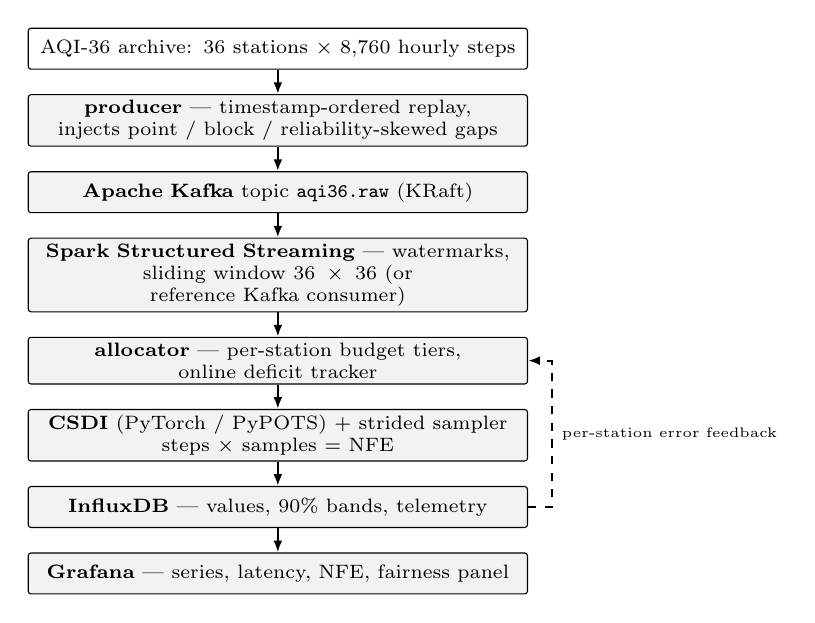
\begin{tikzpicture}[
  node distance=3.1mm,
  box/.style={draw, rounded corners=1pt, align=center, inner sep=2pt,
              minimum height=5.2mm, font=\scriptsize, text width=62mm},
  tool/.style={box, fill=black!5},
  arr/.style={-{Latex[length=1.5mm]}, thick}]
\node[box] (src) {AQI-36 archive: 36 stations $\times$ 8{,}760 hourly steps};
\node[tool, below=of src] (prod) {\textbf{producer} --- timestamp-ordered replay,\\
  injects point / block / reliability-skewed gaps};
\node[tool, below=of prod] (kafka) {\textbf{Apache Kafka} topic \texttt{aqi36.raw} (KRaft)};
\node[tool, below=of kafka] (spark) {\textbf{Spark Structured Streaming} --- watermarks,\\
  sliding window $36\times36$ (or reference Kafka consumer)};
\node[tool, below=of spark] (router) {\textbf{allocator} --- per-station budget tiers,\\
  online deficit tracker};
\node[tool, below=of router] (model) {\textbf{CSDI} (PyTorch / PyPOTS) + strided sampler\\
  steps $\times$ samples = NFE};
\node[tool, below=of model] (influx) {\textbf{InfluxDB} --- values, 90\% bands, telemetry};
\node[tool, below=of influx] (graf) {\textbf{Grafana} --- series, latency, NFE, fairness panel};
\foreach \a/\b in {src/prod, prod/kafka, kafka/spark, spark/router,
                   router/model, model/influx, influx/graf}
  \draw[arr] (\a) -- (\b);
\draw[arr, dashed] (influx.east) -- ++(3mm,0) |- node[right, font=\tiny, pos=0.25]
  {per-station error feedback} (router.east);
\end{tikzpicture}
\caption{The pipeline. Every stage is a distinct tool with real data flowing
between them; the dashed path is the feedback that lets the allocator learn
which stations are being served worst.}
\label{fig:arch}
\end{figure}

Fig.~\ref{fig:arch} shows the system. The brief accepts a Kafka topic replaying
a public dataset as a real stream, which lets us retain ground truth for every
imputed value --- something a live feed cannot provide.

The \textbf{producer} walks the archive in timestamp order at controllable
speed, emitting one message per station per timestep and applying an artificial
missingness process on top of the archive's genuine 13.2\% gaps. Four protocols
are implemented: point (MCAR), block (bursty outage), sensor failure, and
\emph{reliability-skewed}, in which per-station failure probabilities are drawn
from a heavy-tailed distribution so a minority of stations carry most of the
missingness. The last is the realistic case and the one where a dataset-average
metric hides the damage.

The \textbf{stream layer} maintains a sliding window of 36 timesteps across all
36 stations. We provide both a Spark Structured Streaming job and a reference
Kafka consumer; both import the same windowing and imputation modules, so the
two engines cannot drift apart. Spark owns ingestion, watermarking and
micro-batching, and hands each micro-batch to the shared code via
\texttt{foreachBatch}: CSDI needs a contiguous window across all stations, which
per-station stateful operators would fragment.

The \textbf{sink} writes observed values, imputed values, 90\% uncertainty
bands and per-window telemetry (latency, NFE, error on artificially masked
cells) to InfluxDB, which Grafana reads. We use InfluxDB rather than the
TimescaleDB named in our proposal; it is the store in the course's suggested
pipeline and provisions into Grafana with less glue. The storage engine is an
implementation detail and not part of the scientific claim.

\section{Proposed Enhancement}
\label{sec:enh}

\subsection{Making both cost axes free}

CSDI's cost is
\begin{equation}
\mathrm{NFE} = S \times N,
\end{equation}
where $S$ is the number of reverse diffusion steps and $N$ the number of
posterior samples drawn to form the predictive distribution. The reference
configuration uses $S=50$, $N=100$, i.e.\ 5{,}000 network evaluations per
window. PyPOTS fixes $S$ at construction and draws the $N$ samples in a serial
loop, so neither axis can be varied at serving time.

We reimplement the reverse process over the already-trained weights. Steps
become free by DDIM-style strided sampling~\cite{ddim} over the model's own
cumulative-alpha schedule: for a subsequence $\tau$ of timesteps,
\begin{equation}
x_{\tau_{i-1}} = \sqrt{\bar\alpha_{\tau_{i-1}}}\,\hat{x}_0
  + \sqrt{1-\bar\alpha_{\tau_{i-1}}}\;\epsilon_\theta(x_{\tau_i}, \tau_i),
\end{equation}
with $\hat{x}_0 = (x_{\tau_i} - \sqrt{1-\bar\alpha_{\tau_i}}\,\epsilon_\theta)
/\sqrt{\bar\alpha_{\tau_i}}$. Samples become cheap by replicating the batch so
all $N$ are drawn in one pass instead of $N$ passes. Observed cells are clamped
throughout, exactly as in the reference.

We verify this is a faithful generalisation rather than a different model: with
$\tau$ set to the full chain and ancestral updates restored, our sampler
reproduces PyPOTS to within sampling noise (MAE 8.30 vs 8.40, identical CRPS
0.1720), while running 2$\times$ faster from batching alone.

\subsection{Per-gap triage, and how we tested it}

A \emph{gap} is one contiguous run of missing timesteps at one station in one
window. For each gap we extract 17 features computable \emph{before} any
diffusion runs --- gap length and position, the station's recent volatility,
how many geographic neighbours are reporting during the gap, disagreement among
those neighbours, the jump between pre- and post-gap context --- and predict how
much that gap gains from extra compute.

The objective matters. For a fixed gap, the error at the cheapest budget $E_{g,0}$
does not depend on the chosen budget, so
\begin{equation}
\min_{b} \sum_g E_{g,b(g)} \;\equiv\; \max_{b} \sum_g \big(E_{g,0}-E_{g,b(g)}\big),
\label{eq:gain}
\end{equation}
and the $E_{g,0}$ terms cancel. We therefore predict the \emph{gain}
$\Delta_{g,b}=E_{g,0}-E_{g,b}$ directly, enforce monotonicity in cost, and solve
the resulting multiple-choice knapsack by Lagrangian bisection. Predicting
absolute error per budget and differencing two noisy predictions is strictly
worse --- we measured it, and it loses to the uniform knob by 35--50\%.

\subsection{Equity-aware allocation}

Pure expected-gain allocation is regressive: a chronically noisy, chronically
gappy station has low predicted gain, so it is starved forever and the stations
already served worst get worse. We therefore track a decaying per-station error
deficit from the live stream and promote the worst-served fraction to the
expensive budget while the rest receive the cheap one.

\section{Implementation}

The pipeline is Python 3.14 with PyTorch 2.14 (CPU), PyPOTS 1.5, Apache Kafka
3.9 in KRaft mode, Apache Spark 4.2, InfluxDB 2.7 and Grafana 11.3, orchestrated
by Docker Compose. No GPU was available; all results are CPU measurements on a
16-thread AMD Ryzen 7 6800HS.

The baseline is CSDI via PyPOTS with the reference hyperparameters (4 layers,
64 channels, 8 heads, 50 diffusion steps, quadratic $\beta$ schedule from
$10^{-4}$ to $0.5$), 414{,}081 trainable parameters. We follow the CSDI/PriSTI
AQI-36 protocol: 36-step windows, test on months 3, 6, 9 and 12, validate on
months 2, 5, 8 and 11. Training uses a stride-1 sliding view (2{,}917 windows);
evaluation uses non-overlapping windows so each cell is scored once.

The repository separates concerns so that the Spark job and the reference
consumer share code rather than duplicating it: \texttt{stream/windower.py}
holds the sliding-window state, \texttt{models/baseline.py} exposes a frozen
\texttt{train}/\texttt{impute} surface over PyPOTS, \texttt{models/sampler.py}
holds the budget-controllable reverse process, \texttt{router/} holds feature
extraction and allocation, and \texttt{eval/} holds the metrics and the equity
audit. A gate script verifies each link of the chain independently --- dataset,
broker, topic contents, stored values, stored telemetry, checkpoint, model
inference and dashboard --- so a failure names the broken stage rather than the
symptom.

Two implementation details cost us real time and are worth recording. First,
PyPOTS validates by comparing a corrupted series against an intact one; passing
the same array as both yields a validation loss of exactly zero every epoch, so
early stopping fires immediately and the saved ``best'' checkpoint is from epoch
one. Second, CSDI validation runs the full diffusion sampler, so an uncapped
validation set cost 96 minutes per epoch against 65 seconds when capped to 12
windows.

\section{Experimental Setup and Results}
\label{sec:results}

All numbers are on held-out months, scored only on artificially masked cells
where ground truth is known. The router is trained on validation months and
never sees the test split.

\subsection{Baseline reproduction}

Table~\ref{tab:baseline} compares our reproduction against the published
figures. The brief permits ``at least a simplified version'' of the base
method; ours is trained for 16 epochs on a stride-4 view, and reaches the same
order of magnitude. Undercoverage at the 90\% level is expected from a short
run.

\begin{table}[t]
\caption{Baseline CSDI on AQI-36 held-out months (9{,}557 masked cells).}
\label{tab:baseline}
\centering\footnotesize
\begin{tabular}{lrr}
\toprule
Metric & Ours & CSDI published \\
\midrule
MAE ($\mu$g/m$^3$) & 14.43 & 9.51 \\
RMSE & 31.18 & --- \\
MRE & 0.197 & --- \\
CRPS & 0.150 & 0.1056 \\
PICP @ 90\% & 0.794 & --- \\
\bottomrule
\end{tabular}
\end{table}

\subsection{The frontier is dominated by 20 steps}

\begin{figure}[t]
\centering
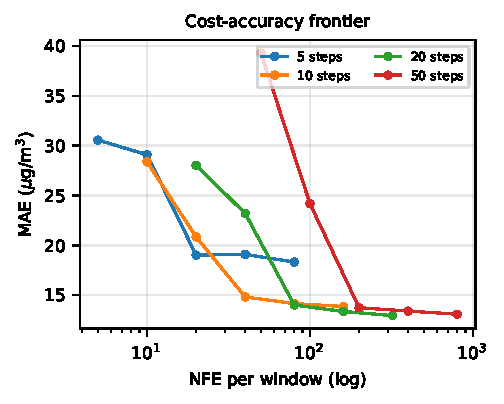
\includegraphics[width=\columnwidth]{figures/pareto.pdf}
\caption{Cost--accuracy frontier over the $(S,N)$ grid. No point on the
frontier uses 50 steps.}
\label{fig:pareto}
\end{figure}

Fig.~\ref{fig:pareto} sweeps $S\in\{2,5,10,20,50\}$ against
$N\in\{1,2,4,8,16\}$. The Pareto frontier never selects 50 steps. Concretely,
$S{=}20,N{=}16$ (320 NFE) reaches MAE 12.95, while $S{=}50,N{=}16$ (800 NFE)
reaches 13.09 --- better accuracy for 2.5$\times$ less compute. At matched
cost the sample axis buys more than the step axis: $20\times8$ (160 NFE, MAE
13.36) beats $50\times4$ (200 NFE, MAE 13.74). This is a pure engineering win
and requires no adaptivity at all.

Table~\ref{tab:sweep} gives the full grid. Two patterns are worth noting
beyond the frontier itself. At $S{=}2$ the reverse process has too few steps to
resolve the data at all and error explodes to several hundred $\mu$g/m$^3$,
which sets a floor on how far the step axis can be pushed regardless of sample
count. And within a fixed step count, CRPS keeps improving with samples long
after MAE has flattened --- at $S{=}20$, MAE moves only from 14.01 to 12.95
between 4 and 16 samples while CRPS improves from 0.2315 to 0.1867. A
point-error metric alone would therefore understate the value of the sample
axis, which is part of why we report both.

\begin{table}[t]
\caption{Full $(S,N)$ sweep on held-out months. Bold marks the Pareto frontier
on (NFE, MAE). Seconds are single-threaded CPU per window.}
\label{tab:sweep}
\centering\footnotesize
\begin{tabular}{rrrrrr}
\toprule
$S$ & $N$ & NFE & MAE & CRPS & s/window \\
\midrule
2 & 1 & 2 & 595.98 & --- & 0.02 \\
2 & 16 & 32 & 458.81 & 6.5309 & 0.86 \\
5 & 1 & \textbf{5} & \textbf{30.56} & --- & 0.05 \\
5 & 4 & \textbf{20} & \textbf{19.02} & 0.3245 & 0.31 \\
5 & 16 & 80 & 18.32 & 0.2972 & 2.05 \\
10 & 1 & \textbf{10} & \textbf{28.37} & --- & 0.10 \\
10 & 4 & \textbf{40} & \textbf{14.82} & 0.2469 & 0.60 \\
10 & 16 & 160 & 13.86 & 0.2013 & 4.24 \\
20 & 4 & \textbf{80} & \textbf{14.01} & 0.2315 & 1.24 \\
20 & 8 & \textbf{160} & \textbf{13.36} & 0.2026 & 3.29 \\
20 & 16 & \textbf{320} & \textbf{12.95} & 0.1867 & 8.41 \\
50 & 4 & 200 & 13.74 & 0.2375 & 3.24 \\
50 & 8 & 400 & 13.40 & 0.2002 & 8.48 \\
50 & 16 & 800 & 13.09 & 0.1891 & 21.24 \\
\bottomrule
\end{tabular}
\end{table}

\subsection{Per-gap triage: a negative result}

An oracle that knows each gap's realised error and allocates optimally appears
to beat the best uniform budget by 49.4\%. That is a large headroom, and it is
almost entirely an artefact.

\begin{figure}[t]
\centering
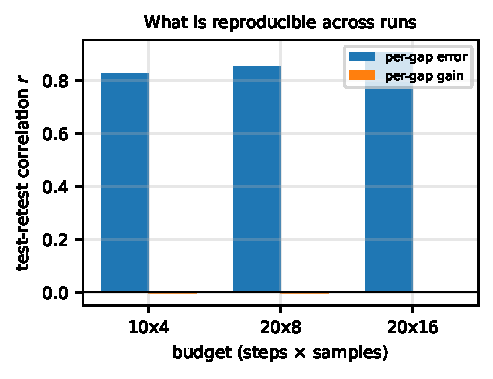
\includegraphics[width=\columnwidth]{figures/reliability.pdf}
\caption{Test--retest correlation across two independent sampling runs at the
same budget. Gap \emph{difficulty} is reproducible; gap \emph{gain} is not.}
\label{fig:rel}
\end{figure}

Diffusion sampling is stochastic: the same gap at the same budget yields
different errors on different runs. Fig.~\ref{fig:rel} measures how much
survives. Per-gap \emph{error} is highly reproducible ($r=0.763$, $0.856$,
$0.913$ at 40, 160 and 320 NFE), so gaps genuinely differ in difficulty. But
per-gap \emph{gain} --- the quantity Eq.~\eqref{eq:gain} requires --- has
$r=0.015$, $0.014$, $0.015$. It is noise.

\begin{figure}[t]
\centering
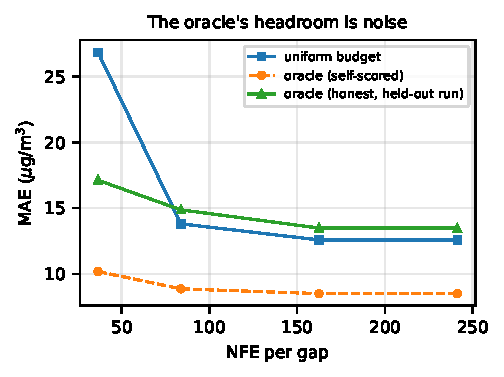
\includegraphics[width=\columnwidth]{figures/oracle.pdf}
\caption{Allocating on one run and scoring on an independent run removes the
oracle's advantage entirely.}
\label{fig:oracle}
\end{figure}

Fig.~\ref{fig:oracle} confirms the consequence. Scoring the oracle on the same
run it was fitted to gives $+32.5\%$ over uniform; scoring the identical
allocation on an independent run gives $-7.2\%$, i.e.\ worse than not adapting
at all. The learned router behaves exactly as this predicts: held-out $R^2$ on
gain is negative at every budget ($-0.098$, $-0.084$, $-0.080$, $-0.088$,
$-0.086$), meaning the model is worse than predicting the mean gain, and the
router underperforms the uniform knob at every budget above the cheapest.

This is not a feature-engineering failure. The features are informative about
\emph{difficulty}: the same gradient-boosted models reach positive $R^2$ when
the target is absolute error rather than gain, and the importances are
physically sensible, led by the pre/post-gap jump, the window and station
missing rates, and neighbour disagreement. The problem is the target. Because
$E_{g,0}$ and $E_{g,b}$ share the gap's systematic difficulty, subtracting them
cancels the signal and leaves the two runs' independent sampling noise.

\subsection{A protocol we would recommend}

The cost of this diagnostic is two sampling runs. Given per-gap errors $A$ and
$B$ from independent runs at each candidate budget, we suggest reporting
(i) $\mathrm{corr}(A_{:,b}, B_{:,b})$, the ceiling on predicting difficulty;
(ii) $\mathrm{corr}(A_{:,0}-A_{:,b},\, B_{:,0}-B_{:,b})$, the ceiling on
predicting gain, which is what an adaptive router actually needs; and
(iii) the honest oracle --- allocate on $A$, score on $B$. Where (ii) is near
zero, no router can succeed and a self-scored oracle will nonetheless promise
large gains.

\subsection{Selective imputation: the asymmetry pays off elsewhere}

The failure above is specific. Gain is unpredictable, but per-gap \emph{error}
is not: the same features reach held-out $R^2=+0.214$ and rank correlation
$+0.403$ when the target is the error itself. That asymmetry closes the door on
adaptive compute and opens a different one. If we can tell which imputations
will be poor, the system can decline to publish them --- and for an alerting
service a missing value is more honest than a confidently wrong one.

\begin{figure*}[t]
\centering
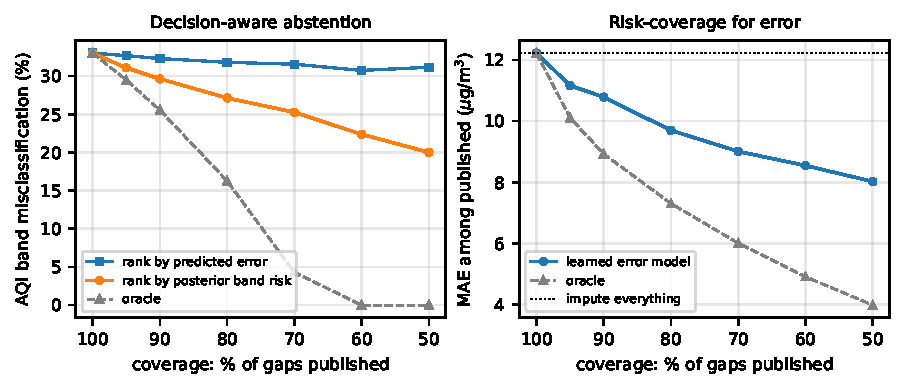
\includegraphics[width=\textwidth]{figures/selective.pdf}
\caption{Left: AQI band misclassification among published values as coverage
falls. Ranking by predicted error magnitude barely helps; ranking by posterior
band risk does. Right: risk--coverage for absolute error.}
\label{fig:selective}
\end{figure*}

Fig.~\ref{fig:selective} (right) shows the risk--coverage trade-off. Withholding
the 20\% of gaps with the highest predicted error cuts MAE among the published
80\% from 12.22 to 9.70, a 20.6\% reduction, capturing 51\% of the reduction an
oracle could achieve.

\textbf{Ranking by error is the wrong criterion for decisions.} Band
misclassification barely moves under that ranking: 33.0\% at full coverage to
31.8\% at 80\%. The reason is structural. A band flip is caused by proximity to
a threshold, not by the magnitude of the error --- a $2\,\mu$g/m$^3$ error at
the 35.4 boundary changes the public-health category, while a
$20\,\mu$g/m$^3$ error mid-band does not.

\textbf{The posterior gives the right criterion directly.} For each imputed
cell we compute the fraction of posterior samples falling in a different AQI
band than the published median,
\begin{equation}
\rho_{i} = \tfrac{1}{N}\textstyle\sum_{j=1}^{N}
\mathbf{1}\!\left[\mathrm{band}(x_i^{(j)}) \neq \mathrm{band}(\hat{x}_i)\right],
\end{equation}
a calibration-free estimate of decision risk that costs nothing extra because
the samples are already drawn. Ranking by $\rho$ rather than by predicted error
cuts band misclassification from 33.0\% to 27.1\% at 80\% coverage and to
20.0\% at 50\% (Table~\ref{tab:selective}) --- relative reductions of 18\% and
39\%, against essentially no movement from the error-based ranking.

\begin{table}[t]
\caption{Band misclassification among published values. Lower is better.}
\label{tab:selective}
\centering\scriptsize
\setlength{\tabcolsep}{4pt}
\begin{tabular}{rrrr}
\toprule
Coverage & by predicted error & by posterior band risk & oracle \\
\midrule
100\% & 33.0\% & 33.0\% & 33.0\% \\
90\%  & 32.3\% & 29.6\% & 25.6\% \\
80\%  & 31.8\% & \textbf{27.1\%} & 16.3\% \\
50\%  & 31.2\% & \textbf{20.0\%} & 0.0\% \\
\bottomrule
\end{tabular}
\end{table}

This is the one place in our study where a \emph{generative} imputer is
decisive. SAITS returns a point estimate and cannot express band risk at all;
$\rho$ exists only because the model returns a posterior. It is also our answer
to what diffusion buys over a cheaper deterministic imputer, which our own cost
measurements otherwise make hard to justify.

\subsection{Equity}

\begin{figure}[t]
\centering
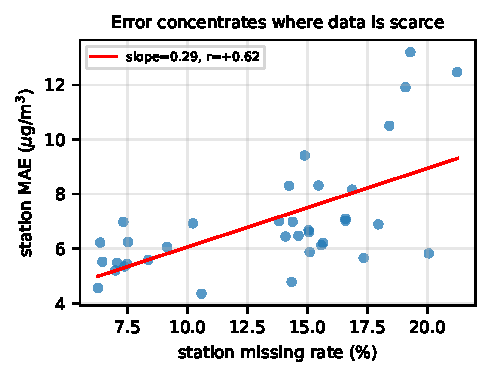
\includegraphics[width=\columnwidth]{figures/equity_scatter.pdf}
\caption{Per-station error against that station's missing rate, baseline model.}
\label{fig:scatter}
\end{figure}

The baseline's headline MAE of 14.43 conceals a 4.2$\times$ spread across
stations: the best is 8.23, the worst 34.44, with an error Gini of 0.176.
Fig.~\ref{fig:scatter} shows why this matters --- error rises with a station's
missing rate (slope $+70.8$, $r=+0.59$). The model is worst exactly where data
is scarcest. Over a quarter of imputed values (27.3\%) fall in the wrong
public-health AQI band.

Because station-level error is reliable, allocation at that level works where
gap-level allocation did not (Table~\ref{tab:equity}). Promoting the worst 30\%
of stations to $20\times16$ and leaving the rest at $10\times4$ costs 126 NFE
on average and achieves an error Gini of 0.155 --- better than giving
\emph{every} station 320 NFE (0.156) --- while capturing 58\% of the
worst-decile improvement for 31\% of the added compute.

\begin{table}[t]
\caption{Station-level allocation at matched cost. Lower is better throughout.}
\label{tab:equity}
\centering\scriptsize
\setlength{\tabcolsep}{3.5pt}
\begin{tabular}{lrrrrr}
\toprule
Variant & NFE & MAE & w-10\% & Gini & band \\
\midrule
uniform cheap ($10{\times}4$) & 40 & 15.30 & 24.00 & 0.166 & 37.2\% \\
uniform rich ($20{\times}16$) & 320 & 13.46 & 21.30 & 0.156 & 32.7\% \\
\textbf{equity mix} & \textbf{126} & 14.76 & 22.44 & \textbf{0.155} & 36.0\% \\
\bottomrule
\end{tabular}
\end{table}

\subsection{In the running system}

With the allocator live in the streaming path the pipeline consumes 217 NFE per
window against the baseline's 400, and the deficit tracker adapts online:
the first window promotes no stations because no error has been observed yet,
and subsequent windows promote 11 of 36.

\section{Discussion}

\textbf{What the negative result means.} Our finding is not that adaptive
compute is a bad idea, but that oracle bounds are a dangerous way to justify it
when the underlying model is stochastic. An oracle fitted to realised errors
absorbs the sampler's noise into its allocation, and reports headroom no
predictor can capture. The diagnostic is cheap --- run the same budget twice
and correlate --- and we would urge it before building any adaptive-computation
router. The distinction that matters is between predicting which inputs are
\emph{hard} (reproducible here, $r\approx0.9$) and which inputs \emph{benefit}
from more compute (not reproducible, $r\approx0.015$).

We also tested the obvious remedy. With $\eta=0$ the DDIM trajectory is
deterministic given the initial latent $x_T$, so fixing $x_T$ across budgets
(common random numbers) removes sampling noise entirely and makes the gain a
deterministic function of the input. It does not help: held-out $R^2$ on gain
falls further, to roughly $-2.0$. The gain is therefore not merely noisy --- it
depends on the interaction between the realised latent and the individual gap,
which no feature of the observed context can see.

\textbf{Threats to validity.} Our baseline is deliberately simplified and its
absolute error is above the published figure; a better-trained model might have
a different noise-to-signal ratio in the gain, although the reliability gap is
so large that the conclusion is unlikely to reverse. Results are on one dataset
with 36 stations. All measurements are CPU-only, so wall-clock latencies are
not representative of GPU deployment --- which is why we report NFE, a
hardware-independent unit, throughout. The equity comparison promotes a fixed
fraction of stations; we did not tune that fraction on test data.

\textbf{On the equity metric.} We do not claim to address environmental
injustice. We claim something narrower and checkable: the evaluation protocol
in current use cannot see this failure mode, and a small change to the reported
metrics makes it visible and improvable.

\section{Conclusion and Future Work}

We built a streaming diffusion imputation pipeline and used it to test per-gap
adaptive computation. The honest answer is that it does not work on AQI-36, and
we showed precisely why: the gain from extra compute is not a reproducible
property of a gap, and fixing the sampler's initial latent across budgets does
not rescue it.

Three useful results survive. Reducing the chain to 20 steps and spending the
budget on posterior samples instead is a 2.5$\times$ saving at better accuracy.
Because per-gap error is predictable even though gain is not, a selective
imputer that abstains on high-risk gaps improves the values it does publish ---
and ranking that abstention by posterior band disagreement rather than by error
magnitude is what makes it matter for the decision a public-health service
actually takes. And moving allocation from gaps to stations --- where the
signal is reliable --- improves the fairness of imputation per unit compute.

Future work should calibrate the abstention threshold against a stated
alert-precision target rather than a fixed coverage; extend the equity allocation to the spatial model
of PriSTI; and evaluate on METR-LA, where $N=207$ makes the $O(N^2d)$ attention
the dominant cost.

\begin{thebibliography}{9}
\bibitem{csdi} Y.~Tashiro, J.~Song, Y.~Song, and S.~Ermon, ``CSDI: Conditional
score-based diffusion models for probabilistic time series imputation,'' in
\emph{Advances in Neural Information Processing Systems (NeurIPS)}, 2021.
\bibitem{pristi} M.~Liu, H.~Huang, H.~Feng, L.~Sun, B.~Du, and Y.~Fu,
``PriSTI: A conditional diffusion framework for spatiotemporal imputation,'' in
\emph{IEEE Int. Conf. on Data Engineering (ICDE)}, 2023, pp.~1927--1939.
\bibitem{saits} W.~Du, D.~C\^{o}t\'{e}, and Y.~Liu, ``SAITS: Self-attention-based
imputation for time series,'' \emph{Expert Systems with Applications}, vol.~219,
p.~119619, 2023.
\bibitem{ddim} J.~Song, C.~Meng, and S.~Ermon, ``Denoising diffusion implicit
models,'' in \emph{Int. Conf. on Learning Representations (ICLR)}, 2021.
\bibitem{stmvl} X.~Yi, Y.~Zheng, J.~Zhang, and T.~Li, ``ST-MVL: Filling missing
values in geo-sensory time series data,'' in \emph{Int. Joint Conf. on
Artificial Intelligence (IJCAI)}, 2016, pp.~2704--2710.
\bibitem{equity} Y.~Sun \emph{et al.}, ``Harmonizing low-cost and regulatory air
quality monitoring networks: reducing exposure misclassification in
underrepresented communities,'' \emph{Journal of Hazardous Materials}, 2025.
\bibitem{pypots} W.~Du, ``PyPOTS: A Python toolbox for data mining on
partially-observed time series,'' \emph{arXiv:2305.18811}, 2023.
\end{thebibliography}

\end{document}
